\section{Assignment B2}

\begin{problem}
    \begin{center}\tikzsetnextfilename{227}
        \begin{tikzpicture}[trim axis left, trim axis right]
            \begin{axis}[
                domain=-4:3,
                samples = 71,
                axis y line=middle,
                axis x line=middle,
                xtick = \empty,
                ytick = \empty,
                xlabel = {$x$},
                ylabel = {$y$},
                ymin=-2,
                ymax=3,
                legend cell align={left},
                legend pos=outer north east,
                after end axis/.code={
                    \path (axis cs:0,0) 
                        node [anchor=north east] {$O$};
                    }
                ]

                \addplot[plotRed] {1/2.6 * x^3 + x^2 + 1};

                \addlegendentry{$y = f(x)$};

                \fill (0, 1) circle[radius=2.5 pt] node[anchor=north east] {$A(0, 1)$};

                \fill (-1.733, 2.001) circle[radius=2.5 pt] node[anchor=south] {$B(-1, 2)$};

                \fill (-2.908, 0) circle[radius=2.5 pt] node[anchor=north west] {$C(-3, 0)$};
            \end{axis}
        \end{tikzpicture}
    \end{center}

    The diagram shows the graph of $y=f(x)$. The points $A$, $B$ and $C$ have coordinates $(0, 1)$, $(-1, 2)$ and $(-3, 0)$ respectively. Sketch, separately, the graphs of
    \begin{enumerate}
        \item $y = f(-x)$
        \item $y = 3 - 2f(x)$
        \item $y = 3f\of{\frac{x}2 + 1}$
    \end{enumerate}
    showing in each case the coordinates of the points corresponding to $A$, $B$ and $C$.
\end{problem}
\begin{solution}
    \begin{ppart}
        \begin{center}\tikzsetnextfilename{228}
            \begin{tikzpicture}[trim axis left, trim axis right]
                \begin{axis}[
                    domain=-3:4,
                    samples = 71,
                    axis y line=middle,
                    axis x line=middle,
                    xtick = \empty,
                    ytick = \empty,
                    xlabel = {$x$},
                    ylabel = {$y$},
                    ymin=-2,
                    ymax=3,
                    legend cell align={left},
                    legend pos=outer north east,
                    after end axis/.code={
                        \path (axis cs:0,0) 
                            node [anchor=north east] {$O$};
                        }
                    ]

                    \addplot[plotRed] {1/2.6 * -x^3 + x^2 + 1};

                    \addlegendentry{$y = f(-x)$};

                    \fill (0, 1) circle[radius=2.5 pt] node[anchor=north east] {$A(0, 1)$};

                    \fill (1.733, 2.001) circle[radius=2.5 pt] node[anchor=south] {$B(1, 2)$};

                    \fill (2.908, 0) circle[radius=2.5 pt] node[anchor=north east] {$C(3, 0)$};
                \end{axis}
            \end{tikzpicture}
        \end{center}
    \end{ppart}
    \begin{ppart}
        \begin{center}\tikzsetnextfilename{229}
            \begin{tikzpicture}[trim axis left, trim axis right]
                \begin{axis}[
                    domain=-4:1,
                    samples = 71,
                    axis y line=middle,
                    axis x line=middle,
                    xtick = \empty,
                    ytick = \empty,
                    xlabel = {$x$},
                    ylabel = {$y$},
                    ymin=-2,
                    ymax=5,
                    legend cell align={left},
                    legend pos=outer north east,
                    after end axis/.code={
                        \path (axis cs:0,0) 
                            node [anchor=north east] {$O$};
                        }
                    ]

                    \addplot[plotRed] {-2*(1/2.6 * x^3 + x^2 + 1)+3};

                    \addlegendentry{$y = 3-2f(x)$};

                    \fill (0, 1) circle[radius=2.5 pt] node[anchor=south east] {$A(0, 1)$};

                    \fill (-1.733, -1) circle[radius=2.5 pt] node[anchor=north] {$B(-1, 2)$};

                    \fill (-2.908, 3) circle[radius=2.5 pt] node[anchor=west] {$C(-3, 3)$};
                \end{axis}
            \end{tikzpicture}
        \end{center}
    \end{ppart}
    \begin{ppart}
        \begin{center}\tikzsetnextfilename{230}
            \begin{tikzpicture}[trim axis left, trim axis right]
                \begin{axis}[
                    domain=-9:4,
                    samples = 71,
                    axis y line=middle,
                    axis x line=middle,
                    xtick = \empty,
                    ytick = \empty,
                    xlabel = {$x$},
                    ylabel = {$y$},
                    ymin=-3,
                    ymax=15,
                    legend cell align={left},
                    legend pos=outer north east,
                    after end axis/.code={
                        \path (axis cs:0,0) 
                            node [anchor=north east] {$O$};
                        }
                    ]

                    \addplot[plotRed] {3* (1/2.6 * (x/2 + 1)^3 + (x/2 + 1)^2 + 1)};

                    \addlegendentry{$y = 3f(\frac{x}2 - 1)$};

                    \fill (-2, 3) circle[radius=2.5 pt] node[anchor=north] {$A(-2, 3)$};

                    \fill (-5.467,6.004) circle[radius=2.5 pt] node[anchor=south] {$B(-4, 6)$};

                    \fill (-7.815, 0) circle[radius=2.5 pt] node[anchor=north west] {$C(-8, 0)$};
                \end{axis}
            \end{tikzpicture}
        \end{center}
    \end{ppart}
\end{solution}

\begin{problem}
    \begin{center}\tikzsetnextfilename{231}
        \begin{tikzpicture}[trim axis left, trim axis right]
            \begin{axis}[
                domain=-2:2.5,
                samples = 131,
                axis y line=middle,
                axis x line=middle,
                xtick = {-1, 0, 2},
                ytick = \empty,
                xlabel = {$x$},
                ylabel = {$y$},
                ymin=-3,
                ymax=4,
                legend cell align={left},
                legend pos=outer north east,
                after end axis/.code={
                    \path (axis cs:0,0) 
                        node [anchor=north east] {$O$};
                    }
                ]

                \addplot[plotRed] {-1 * x^2 * (x+1) * (x-2)^3};

                \addlegendentry{$y = f(x)$};

                \fill (-0.737, 2.929) circle[radius=2.5 pt] node[anchor=south] {$(-\frac34, 3)$};

                \fill (0.904, 2.048) circle[radius=2.5 pt] node[anchor=south] {$(1, 2)$};
            \end{axis}
        \end{tikzpicture}
    \end{center}

    The curve shown is the graph of $y = f(x)$. The $x$-axis is a tangent at the origin and at $(2, 0)$. The curve has two maximum points at $\bp{-\frac34, 3}$ and $(1, 2)$. On two separate diagrams, sketch the graphs of the following equations. Show clearly the shapes of the graphs where they meet the $x$-axis and any asymptotes.

    \begin{enumerate}
        \item $y = \frac1{f(x)}, \, x \neq -1, 0, 2$
        \item $y = f(\abs{x})$
    \end{enumerate}
\end{problem}
\begin{solution}
    \begin{ppart}
        \begin{center}\tikzsetnextfilename{232}
            \begin{tikzpicture}[trim axis left, trim axis right]
                \begin{axis}[
                    domain=-2:2.5,
                    samples = 91,
                    axis y line=middle,
                    axis x line=middle,
                    xtick = \empty,
                    ymin=-5,
                    ymax=9,
                    ytick = \empty,
                    xlabel = {$x$},
                    ylabel = {$y$},
                    legend cell align={left},
                    legend pos=outer north east,
                    after end axis/.code={
                        \path (axis cs:0,0) 
                            node [anchor=south east] {$O$};
                        }
                    ]

                    \addplot[plotRed, unbounded coords=jump] {1/(-1 * x^2 * (x+1) * (x-2)^3)};

                    \addplot[plotRed, unbounded coords=jump, samples=81, domain=-1.1:-0.9] {1/(-1 * x^2 * (x+1) * (x-2)^3)};

                    \addlegendentry{$y = \frac1{f(x)}$};

                    \fill (-0.737, 0.341) circle[radius=2.5 pt];
                    
                    \node[anchor=north] at (-0.5, 0) {$(-\frac34, \frac13)$};

                    \fill (0.904, 0.488) circle[radius=2.5 pt] node[anchor=south] {$(1, \frac12)$};

                    \draw[dotted, thick] (-1, 9) -- (-1, -5) node[anchor=south east] {$x = -1$};

                    \draw[dotted, thick] (2, 9) -- (2, -5) node[anchor=south east] {$x = 2$};
                \end{axis}
            \end{tikzpicture}
        \end{center}
    \end{ppart}
    \begin{ppart}
        \begin{center}\tikzsetnextfilename{233}
            \begin{tikzpicture}[trim axis left, trim axis right]
                \begin{axis}[
                    domain=-2.5:2.5,
                    samples = 131,
                    axis y line=middle,
                    axis x line=middle,
                    xtick = {-2, 0, 2},
                    ytick = \empty,
                    xlabel = {$x$},
                    ylabel = {$y$},
                    ymin=-3,
                    ymax=4,
                    legend cell align={left},
                    legend pos=outer north east,
                    after end axis/.code={
                        \path (axis cs:0,0) 
                            node [anchor=north east] {$O$};
                        }
                    ]

                    \addplot[plotRed] {-1 * x^2 * (abs(x)+1) * (abs(x)-2)^3};

                    \addlegendentry{$y = f(\abs{x})$};

                    \fill (-0.904, 2.048) circle[radius=2.5 pt] node[anchor=south] {$(-1, 2)$};

                    \fill (0.904, 2.048) circle[radius=2.5 pt] node[anchor=south] {$(1, 2)$};
                \end{axis}
            \end{tikzpicture}
        \end{center}
    \end{ppart}
\end{solution}

\begin{problem}
    A graph with equation $y = f(x)$ undergoes transformation $A$ followed by transformation $B$ where $A$ and $B$ are described as follows:

    \begin{itemize}
        \item $A$: a translation of 1 unit in the positive direction of the $x$-axis
        \item $B$: a scaling parallel to the $x$-axis by a factor $\frac12$
    \end{itemize}

    The resulting equation is $y = 4x^2-4x+1$. Find the equation $y = f(x)$.
\end{problem}
\begin{solution}
    Note that
    \begin{alignat*}{2}
        &A \colon x \mapsto x-1 &&\implies A^{-1} \colon x \mapsto x+1\\
        &B \colon x \mapsto 2x &&\implies B^{-1} \colon x \mapsto \frac12 x.
    \end{alignat*}

    Hence,
    \begin{center}\tikzsetnextfilename{234}
        \begin{tikzpicture}
            \node (F) {$y = 4x^2-4x+1$};
            \node[below of=F, yshift=-1cm] (B) {$y = 4\bp{\dfrac12 x}^2-4\bp{\dfrac12 x}+1$};
            \node[below of=B, yshift=-1.5cm] (A) {$y = 4\bs{\dfrac12 (x+1)}^2-4\bs{\dfrac12 (x+1)}+1$};

            \draw[->] (F) -- node[anchor=west] {$B^{-1}$} (B);
            \draw[->] (B) -- node[anchor=west] {$A^{-1}$} (A);
        \end{tikzpicture}
    \end{center}

    Observe that $y$ simplifies to \[y = 4\bs{\frac12 (x+1)}^2-4\bs{\frac12 (x+1)}+1 = (x+1)^2-2(x+1)+1 = x^2 + 2x + 1 - 2x - 2 + 1 = x^2.\]
\end{solution}